%----------------------------------------------------------------------------------------
%	PACKAGES AND OTHER DOCUMENT CONFIGURATIONS
%----------------------------------------------------------------------------------------

\documentclass[11pt]{article}

%----------------------------------------------------------------------------------------
%	PACKAGES AND OTHER DOCUMENT CONFIGURATIONS
%----------------------------------------------------------------------------------------

\usepackage{lastpage} % Required to determine the last page number for the footer

\usepackage{multicol}

\usepackage{nth}

\usepackage{graphicx} % Required to insert images

\setlength\parindent{0pt} % Removes all indentation from paragraphs

\usepackage[most]{tcolorbox} % Required for boxes that split across pages

\usepackage{booktabs} % Required for better horizontal rules in tables

\usepackage{listings} % Required for insertion of code

\usepackage{etoolbox} % Required for if statements

%----------------------------------------------------------------------------------------
%	MARGINS
%----------------------------------------------------------------------------------------

\usepackage{geometry} % Required for adjusting page dimensions and margins

\geometry{
	paper=a4paper, % Change to letterpaper for US letter
	top=3cm, % Top margin
	bottom=3cm, % Bottom margin
	left=2.5cm, % Left margin
	right=2.5cm, % Right margin
	headheight=14pt, % Header height
	footskip=1.4cm, % Space from the bottom margin to the baseline of the footer
	headsep=1.2cm, % Space from the top margin to the baseline of the header
	%showframe, % Uncomment to show how the type block is set on the page
}

%----------------------------------------------------------------------------------------
%	FONT
%----------------------------------------------------------------------------------------

\usepackage[utf8]{inputenc} % Required for inputting international characters
\usepackage[T1]{fontenc} % Output font encoding for international characters

\usepackage[sfdefault,light]{roboto} % Use the Roboto font

%----------------------------------------------------------------------------------------
%	HEADERS AND FOOTERS
%----------------------------------------------------------------------------------------

\usepackage{fancyhdr} % Required for customising headers and footers

\pagestyle{fancy} % Enable custom headers and footers

\lhead{\assignmentTitle} % Left header; output the instructor in brackets if one was set
\chead{} % Centre header
\rhead{\assignmentAuthorName} % Right header; output the author name if one was set, otherwise the due date if that was set

\lfoot{} % Left footer
\cfoot{\small Page\ \thepage\ of\ \pageref{LastPage}} % Centre footer
\rfoot{} % Right footer

\renewcommand\headrulewidth{0.5pt} % Thickness of the header rule

%----------------------------------------------------------------------------------------
%	MODIFY SECTION STYLES
%----------------------------------------------------------------------------------------

\usepackage{titlesec} % Required for modifying sections

%------------------------------------------------
% Section

\titleformat
{\section} % Section type being modified
[block] % Shape type, can be: hang, block, display, runin, leftmargin, rightmargin, drop, wrap, frame
{\Large\bfseries} % Format of the whole section
{\assignmentQuestionName~\thesection} % Format of the section label
{6pt} % Space between the title and label
{} % Code before the label

\titlespacing{\section}{0pt}{0.5\baselineskip}{0.5\baselineskip} % Spacing around section titles, the order is: left, before and after

%------------------------------------------------
% Subsection

\titleformat
{\subsection} % Section type being modified
[block] % Shape type, can be: hang, block, display, runin, leftmargin, rightmargin, drop, wrap, frame
{\itshape} % Format of the whole section
{(\alph{subsection})} % Format of the section label
{4pt} % Space between the title and label
{} % Code before the label

\titlespacing{\subsection}{0pt}{0.5\baselineskip}{0.5\baselineskip} % Spacing around section titles, the order is: left, before and after

\renewcommand\thesubsection{(\alph{subsection})}

%----------------------------------------------------------------------------------------
%	CUSTOM QUESTION COMMANDS/ENVIRONMENTS
%----------------------------------------------------------------------------------------

% Environment to be used for each question in the assignment
\newenvironment{question}{
	\vspace{0.5\baselineskip} % Whitespace before the question
	\section{} % Blank section title (e.g. just Question 2)
	\lfoot{\small\itshape\assignmentQuestionName~\thesection~continued on next page\ldots} % Set the left footer to state the question continues on the next page, this is reset to nothing if it doesn't (below)
}{
	\lfoot{} % Reset the left footer to nothing if the current question does not continue on the next page
}

%------------------------------------------------

% Environment for subquestions, takes 1 argument - the name of the section
\newenvironment{subquestion}[1]{
	\subsection{#1}
}{
}

%------------------------------------------------

% Command to print a question sentence
\newcommand{\questiontext}[1]{
	\textbf{#1}
	\vspace{0.5\baselineskip} % Whitespace afterwards
}

%------------------------------------------------

% Command to print a box that breaks across pages with the question answer
\newcommand{\answer}[1]{
	\begin{tcolorbox}[breakable, enhanced]
		#1
	\end{tcolorbox}
}

%------------------------------------------------

% Command to print a box that breaks across pages with the space for a student to answer
\newcommand{\answerbox}[1]{
	\begin{tcolorbox}[breakable, enhanced]
		\vphantom{L}\vspace{\numexpr #1-1\relax\baselineskip} % \vphantom{L} to provide a typesetting strut with a height for the line, \numexpr to subtract user input by 1 to make it 0-based as this command is
	\end{tcolorbox}
}

%------------------------------------------------

% Command to print an assignment section title to split an assignment into major parts
\newcommand{\assignmentSection}[1]{
	{
		\centering % Centre the section title
		\vspace{2\baselineskip} % Whitespace before the entire section title
		
		\rule{0.8\textwidth}{0.5pt} % Horizontal rule
		
		\vspace{0.75\baselineskip} % Whitespace before the section title
		{\LARGE \MakeUppercase{#1}} % Section title, forced to be uppercase
		
		\rule{0.8\textwidth}{0.5pt} % Horizontal rule
		
		\vspace{\baselineskip} % Whitespace after the entire section title
	}
}

%----------------------------------------------------------------------------------------
%	TITLE PAGE
%----------------------------------------------------------------------------------------

\author{\textbf{\assignmentAuthorName}} % Set the default title page author field
\date{} % Don't use the default title page date field

\title{
	\thispagestyle{empty} % Suppress headers and footers
	\vspace{0.2\textheight} % Whitespace before the title
	\textbf{\assignmentTitle}\\[-4pt]
	\ifdef{\assignmentDueDate}{{\small Due\ on\ \assignmentDueDate}\\}{} % If a due date is supplied, output it
	\ifdef{\assignmentClassInstructor}{{\large \textit{\assignmentClassInstructor}}}{} % If an instructor is supplied, output it
	\vspace{0.32\textheight} % Whitespace before the author name
}
 % Include the file specifying the document structure and custom commands

%----------------------------------------------------------------------------------------
%	ASSIGNMENT INFORMATION
%----------------------------------------------------------------------------------------

% Required
\newcommand{\assignmentQuestionName}{Part} % The word to be used as a prefix to question numbers; example alternatives: Problem, Exercise
\newcommand{\assignmentClass}{} % Course/class
\newcommand{\assignmentTitle}{America's Secret War against Bolshevism:\\ U.S. Intervention in the Russian Civil War — Handout} % Assignment title or name
\newcommand{\assignmentAuthorName}{Michael Brodskiy} % Student name



\begin{document}


\maketitle % Print the title page

\thispagestyle{empty} % Suppress headers and footers on the title page

\newpage

\begin{multicols}{2}

\begin{center}
  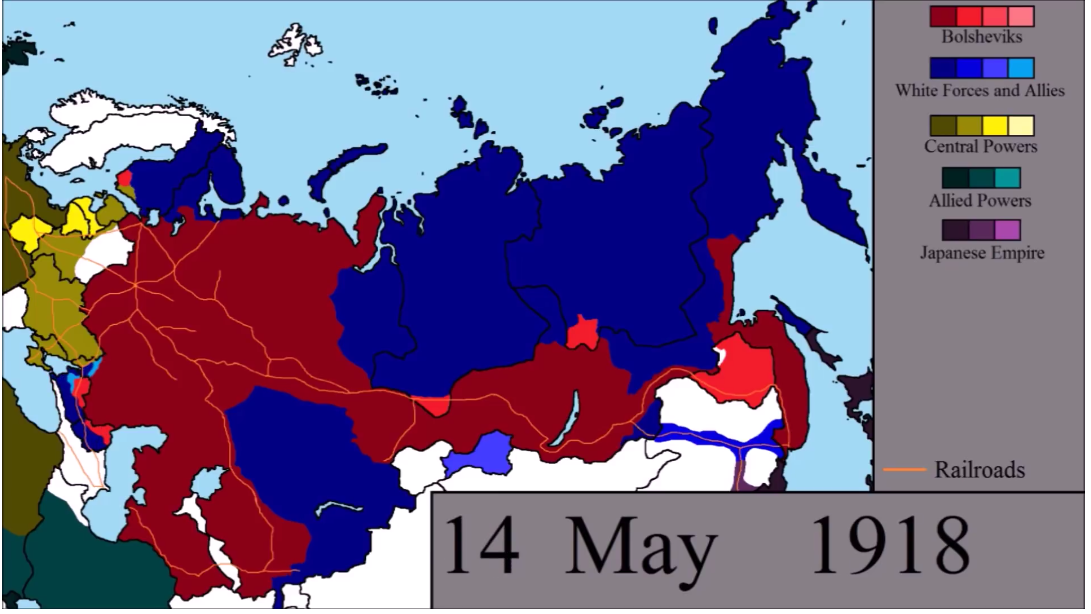
\includegraphics[width=0.95\columnwidth]{images/1918.png}
\end{center}
\begin{center}
  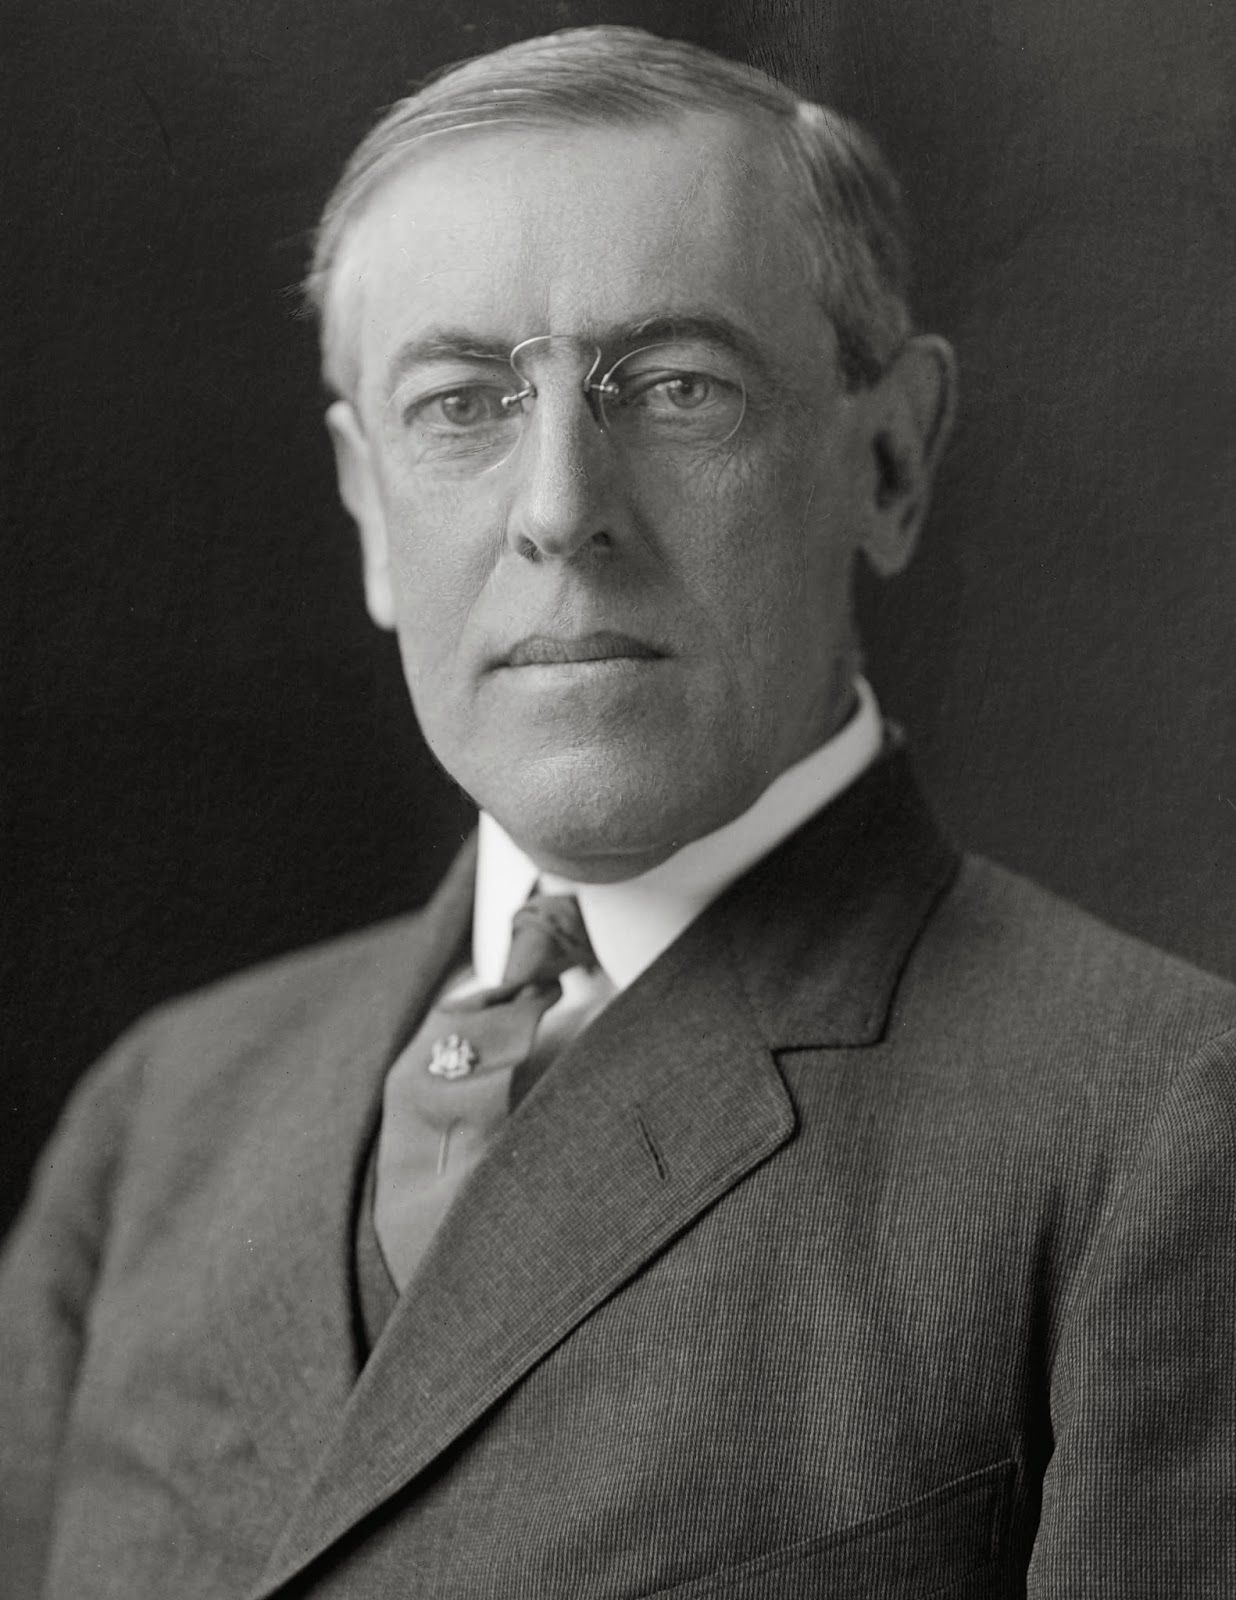
\includegraphics[width=.475\columnwidth]{images/Wilson.png}
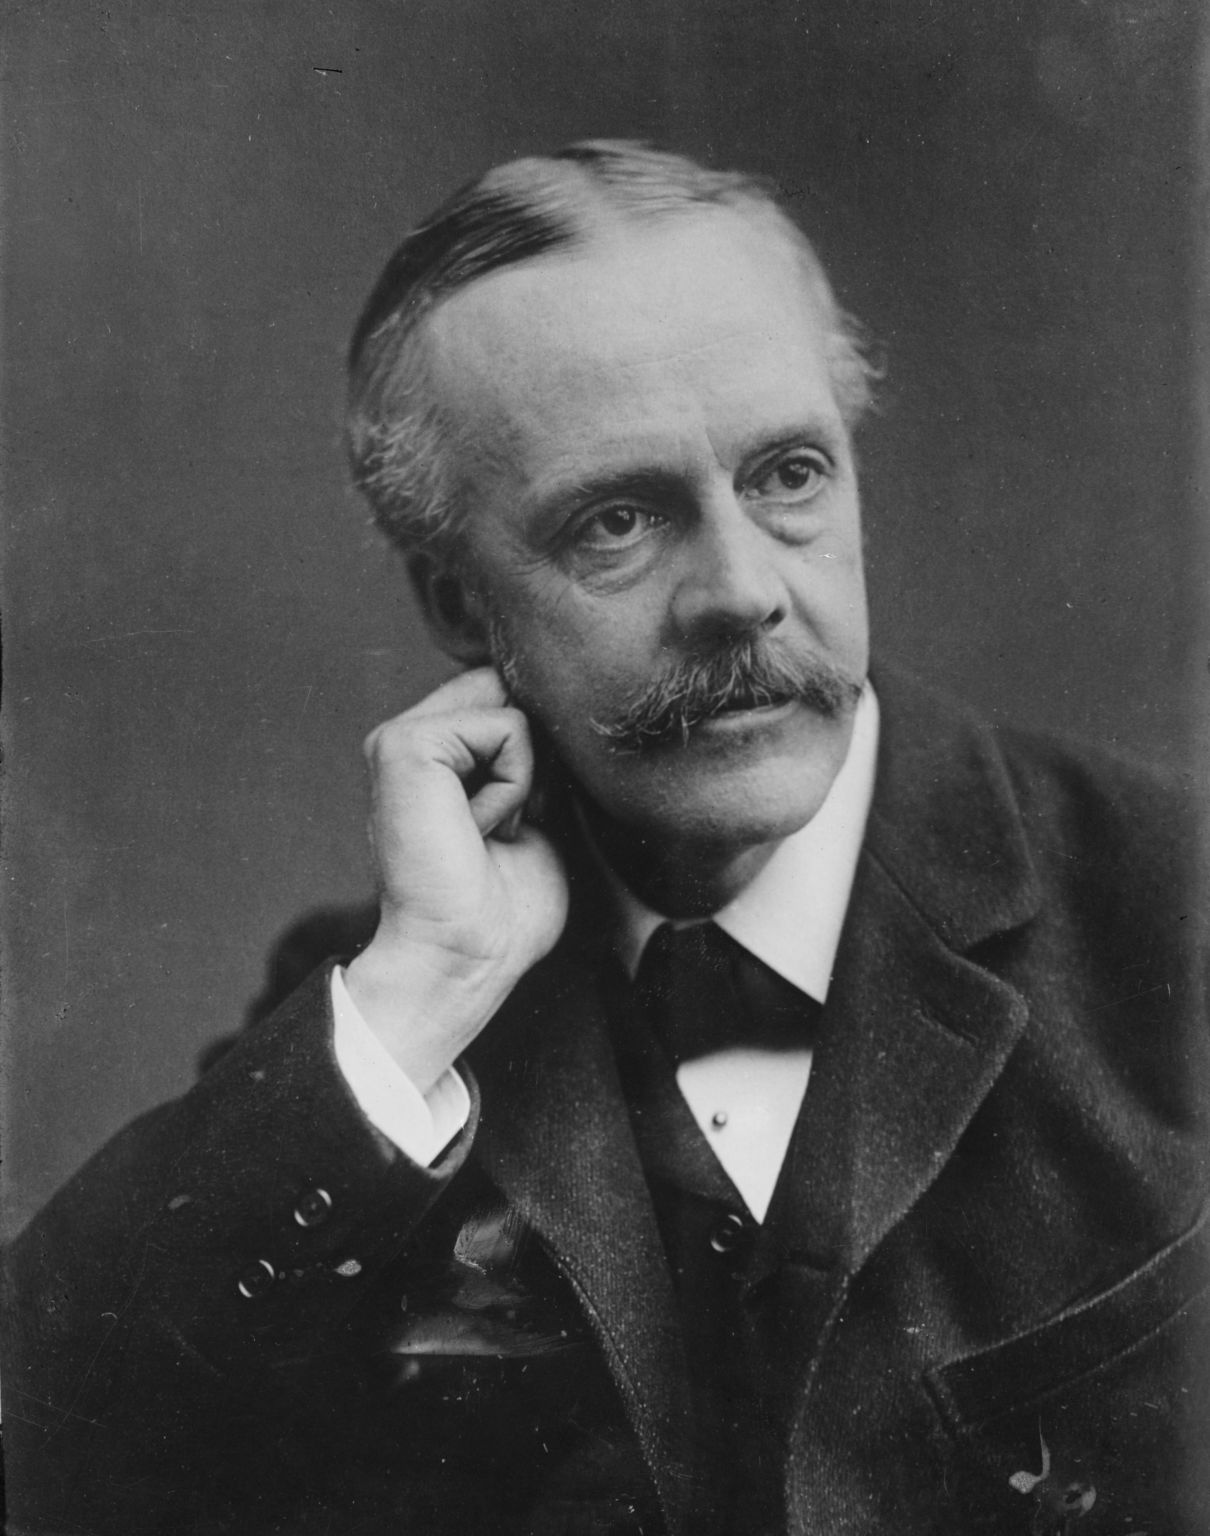
\includegraphics[width=.475\columnwidth]{images/Balfour.png}
\end{center}

\answer{\begin{center} \underline{Context} \vspace{-10pt}  \end{center}\begin{itemize} \item Towards end of first World War, Russia was plunged into revolution and subsequent civil war \item Russia gave significant territory to Germany to leave peacefully (Brest-Litovsk Treaty) \item \textit{Bolsheviki} (pro-Leninist ``reds'') were at war with anti-Bolshevik forces (monarchist ``whites'' and agrarian ``greens'') \item Worry of German spread to port cities of Arkhangelsk and Murmansk \item It was time for Allies to shift policy  \end{itemize}}

\end{multicols}


\begin{multicols}{2}

  \answer{\begin{center} \underline{Important Documents and Figures}  \end{center} \vspace{-10pt} \begin{itemize} \item Supreme War Council (SWC) — An American military headquarters based in Europe and established after the Russian Revolution to more easily control American military policy \item Woodrow Wilson was the American President \begin{itemize} \item Joint Note 31 was approved by the SWC, and justified intervention \item \textit{Aide Memoire} was an attempt by Wilson to define American stance on intervention  \end{itemize} \item Trotsky, part of the ``revolutionary trio'' with Stalin and Lenin, would come to head the Red Army \item Arthur Balfour was the British Foreign Secretary  \item Remember, this work refers to \textbf{\underline{North Russia}}, not Siberia (though intervention occurred there too)\end{itemize}}

  \begin{multicols}{2}
    \begin{center}
    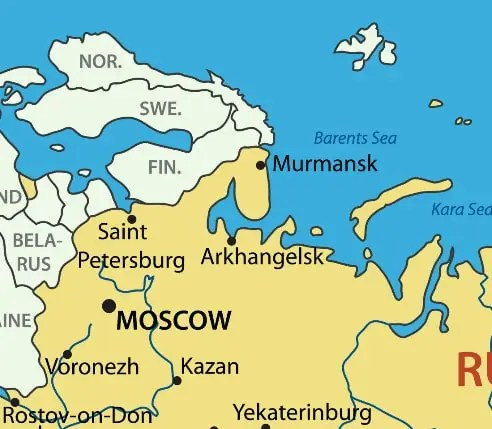
\includegraphics[width=.9\columnwidth]{images/Expedition.png}\\
    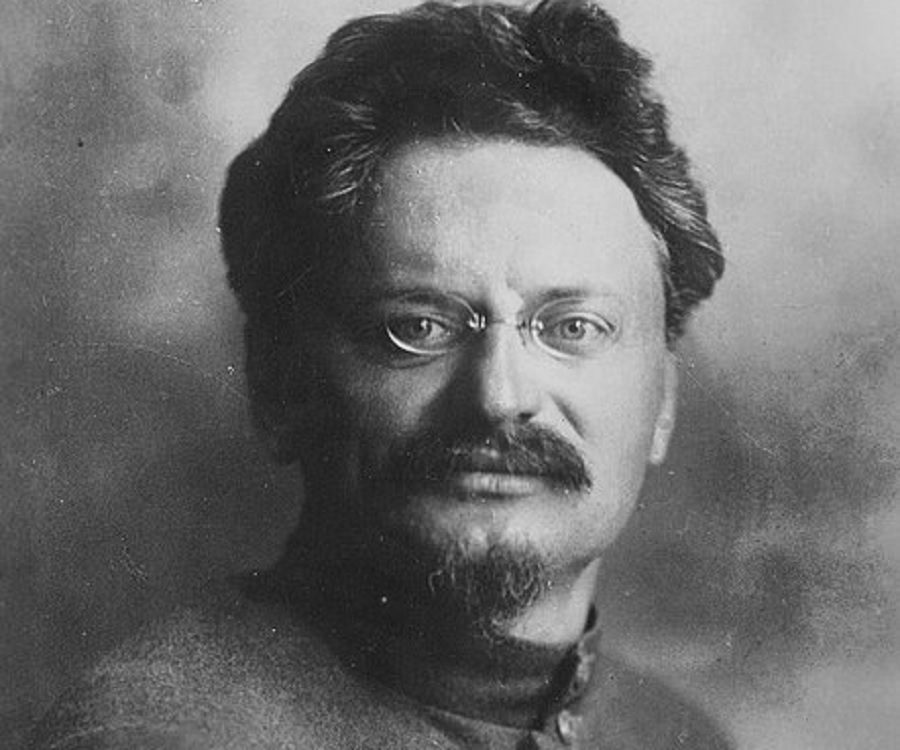
\includegraphics[width=.9\columnwidth]{images/Trotsky.png}
    \end{center}
    \begin{center}
    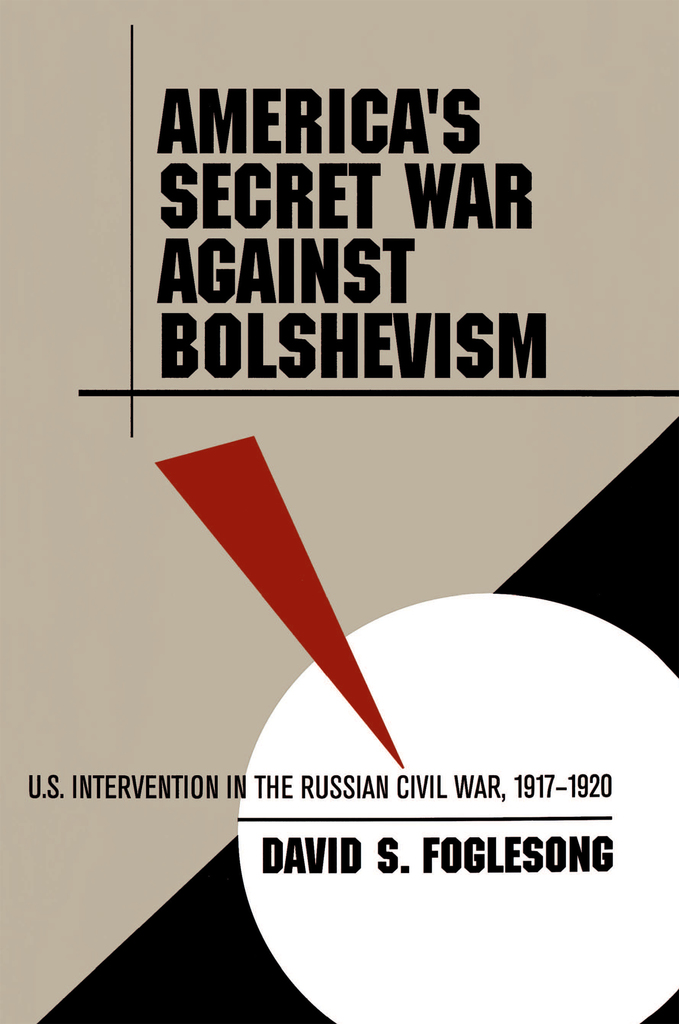
\includegraphics[width=.975\columnwidth]{images/cover.png}
  \end{center}
  \end{multicols}

  \vspace{-39pt}

  \begin{center}
    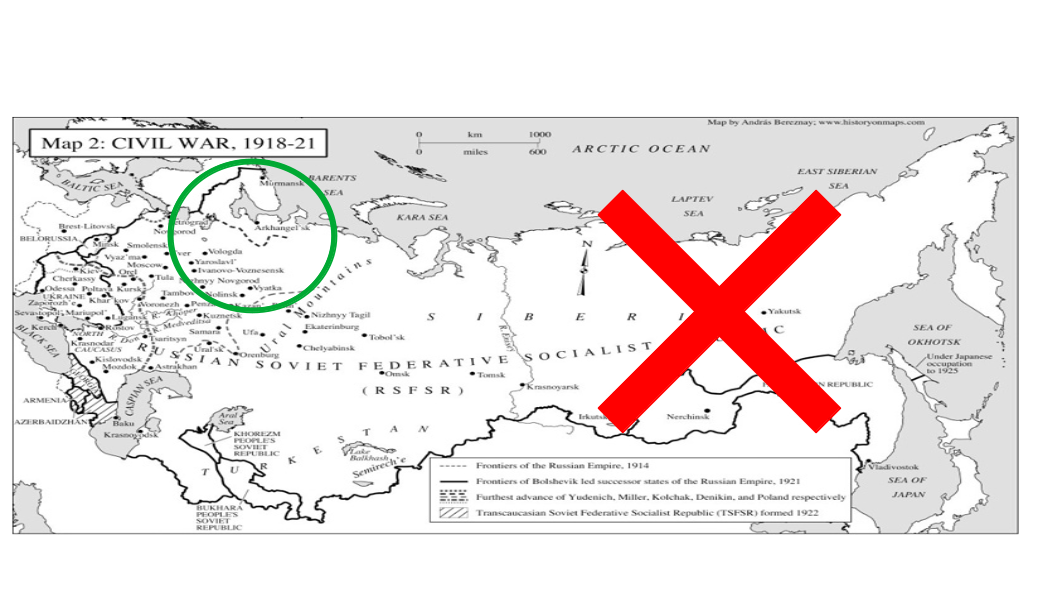
\includegraphics[width=.95\columnwidth]{images/combined.png}\\
    \vspace{-10pt}
    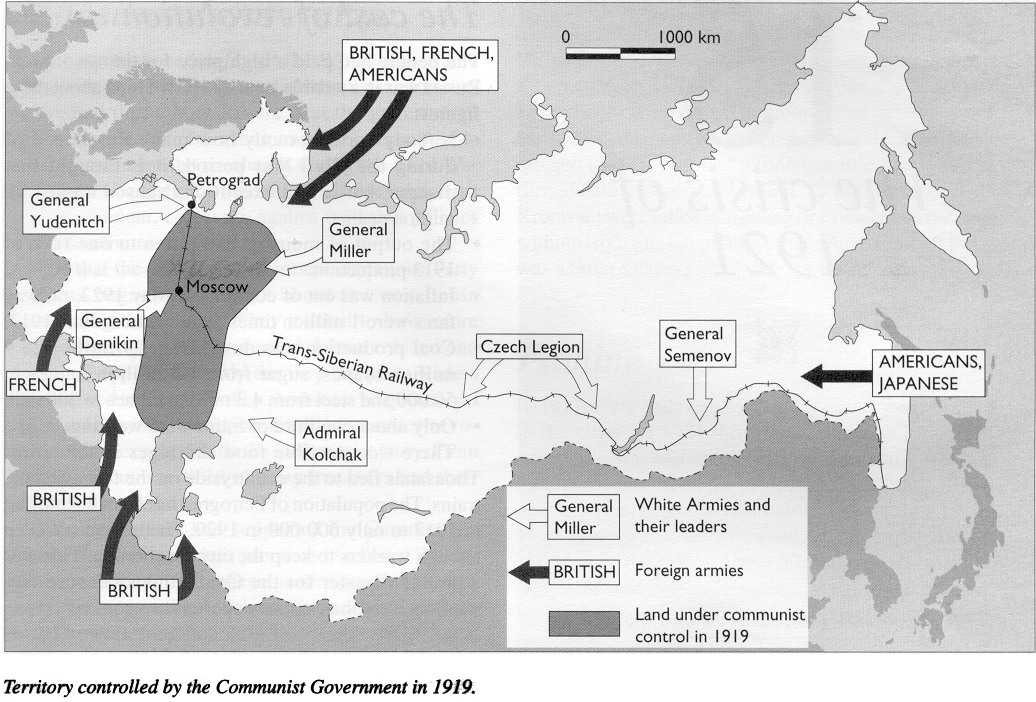
\includegraphics[width=.95\columnwidth]{images/map.png}
  \end{center}

\end{multicols}

\vspace{-30pt}

\begin{multicols}{2}

  \answer{\begin{itemize} \item Wilson wanted intervention, but feared Soviet reaction and/or reprisal \begin{itemize} \item Possible nationalistic uprising in response \end{itemize} \item “When Wilson agreed to send American soldiers to Archangel, then, he sought not only to conciliate his Allies, but also to help the Russian people liberate their country from an allegedly alien and tyrannical regime.” \end{itemize}}

  \begin{center}
    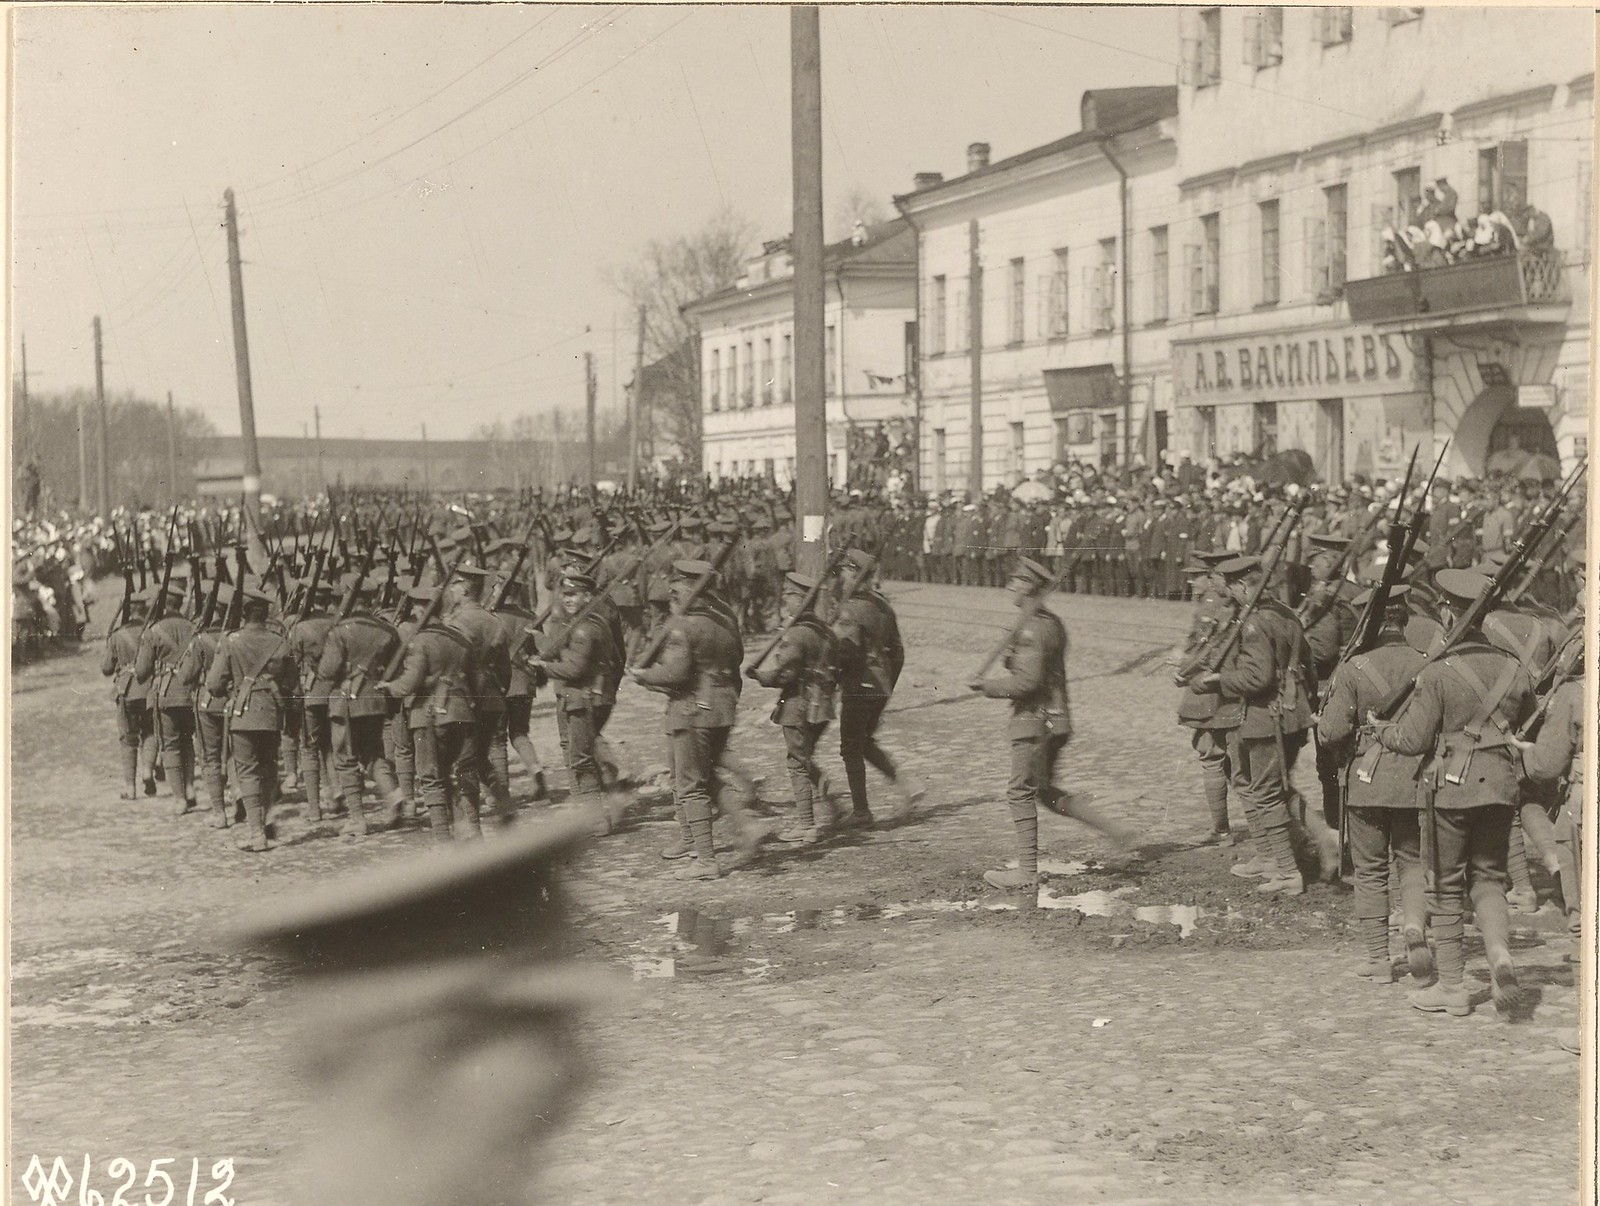
\includegraphics[width=.95\columnwidth]{images/BritishPatrol.png}
  \end{center}


\end{multicols}

\vspace{-40pt}

\assignmentSection{Escalation}

\vspace{-15pt}

\begin{multicols}{2}

\begin{center}
  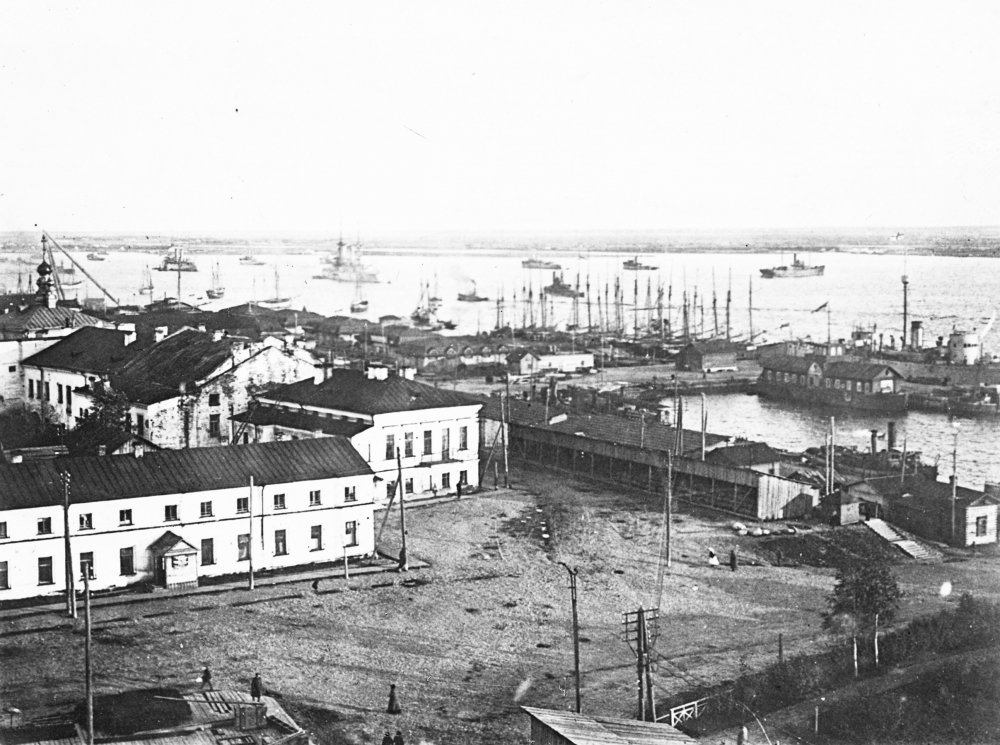
\includegraphics[width=.95\columnwidth]{images/Murmansk1918.png}
\end{center}

\answer{\begin{itemize} \item On May 31, Balfour urged Americans that it was of great importance, “to retain Murmansk, if we desire to retain any possibility at all of entering Russia” \item On June 1, Wilson reiterated that he “was entirely willing to send troops to Murmansk,” but he took no action until later \end{itemize}}

\end{multicols}

\vspace{-10pt}

\begin{multicols}{2}

  \answer{\begin{itemize} \item On June 3, Joint Note 31 was approved by the Supreme War Council, stated: \begin{itemize} \item Allied intervention in north Russia was justified because of German threat \item Also because “the majority of Russian parties” had requested it  \end{itemize}\end{itemize}}

\begin{center}
  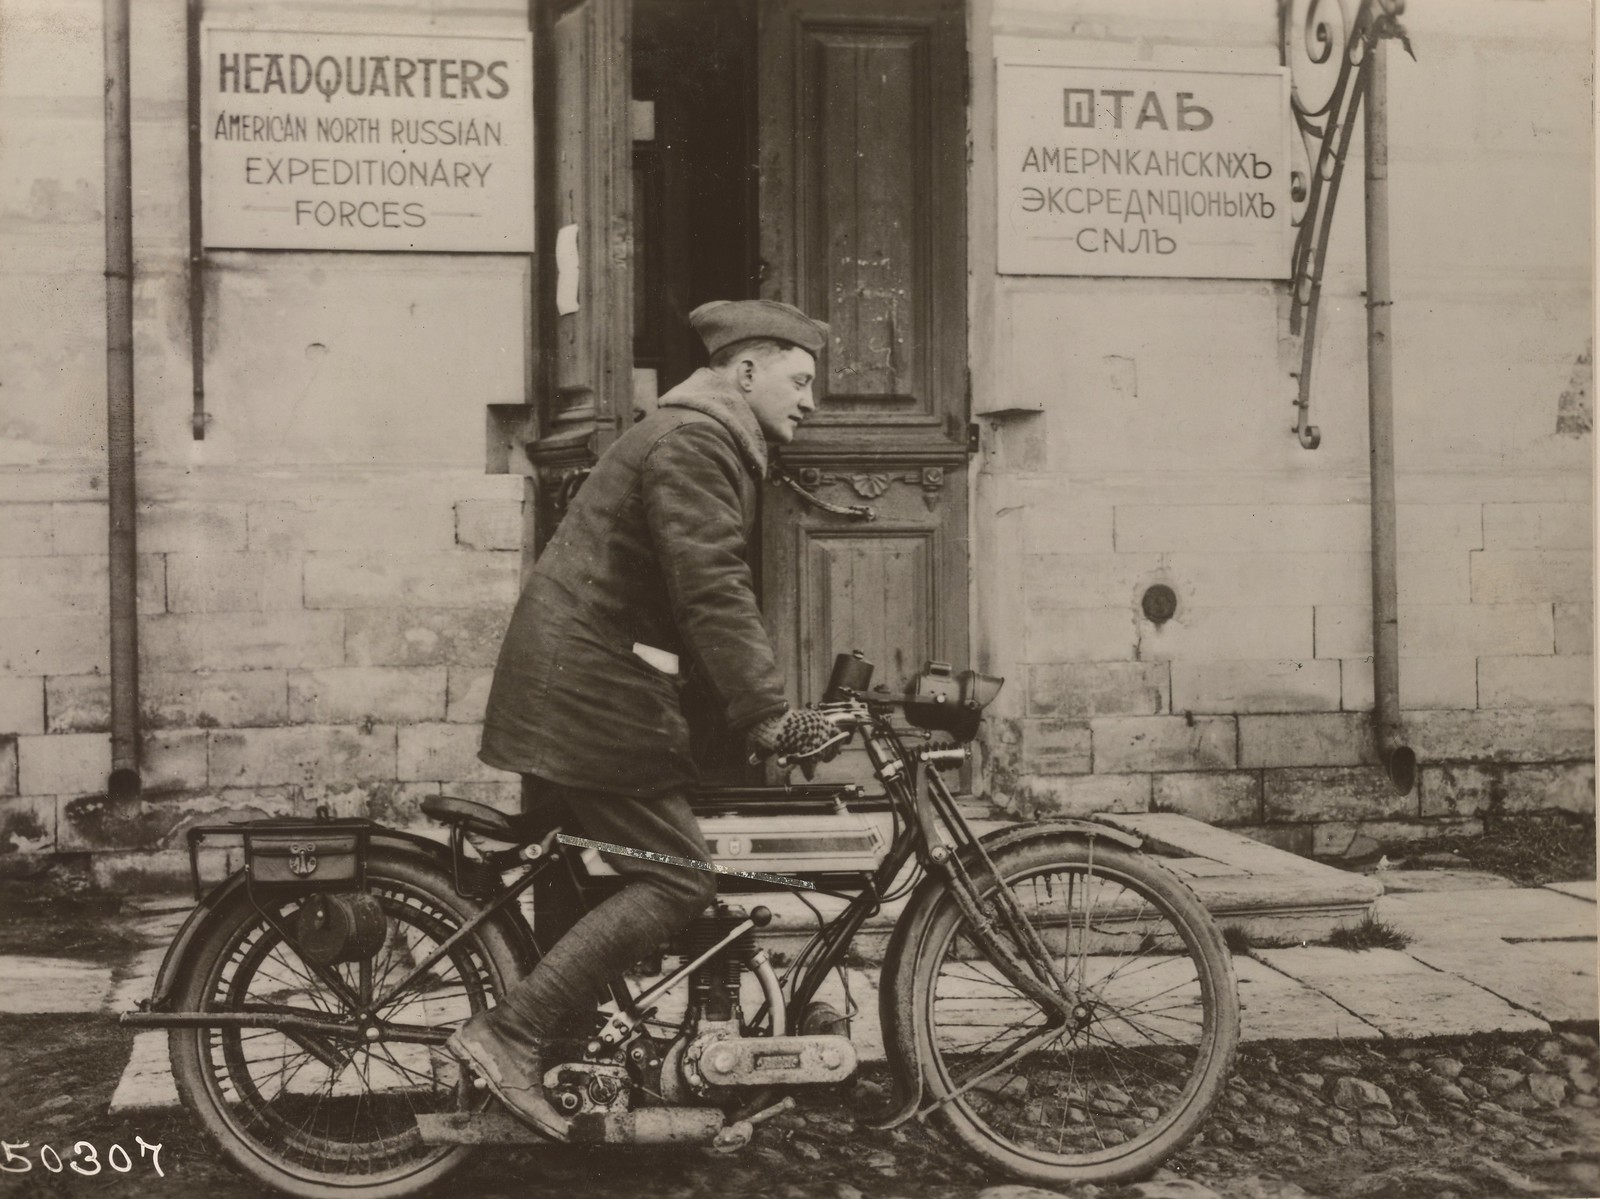
\includegraphics[width=.95\columnwidth]{images/HQ.png}
\end{center}

\end{multicols}

\vspace{-25pt}

\begin{multicols}{2}

  \answer{\begin{itemize} \item Allied supplies piled up in the Soviet port cities \vspace{-5pt} \item July 1918, Wilson releases \textit{aide memoire}\end{itemize}}

  \answer{\vspace{-10pt} \begin{itemize} \item 339th Infantry Regiment was to be dispatched \vspace{-10pt} \item "to guard military stores which may subsequently be needed by Russian forces . . ." \end{itemize}}

\end{multicols}

\begin{multicols}{2}

  \begin{center}
    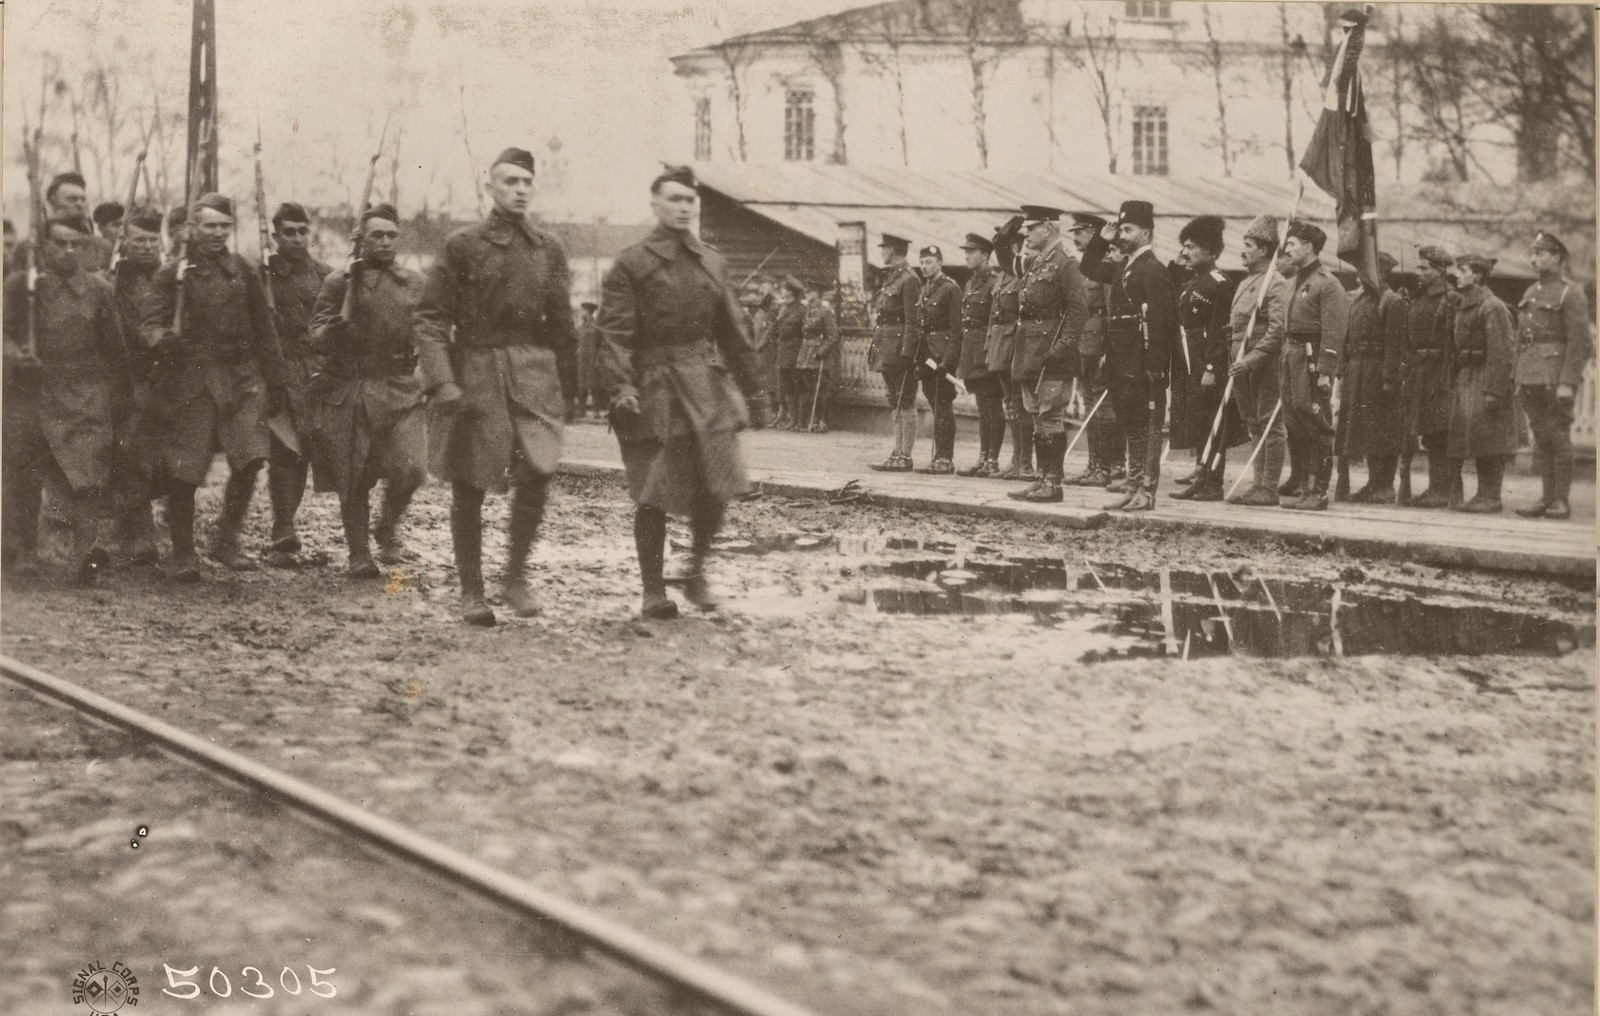
\includegraphics[width=.95\columnwidth]{images/AmericanParade.png} \\
    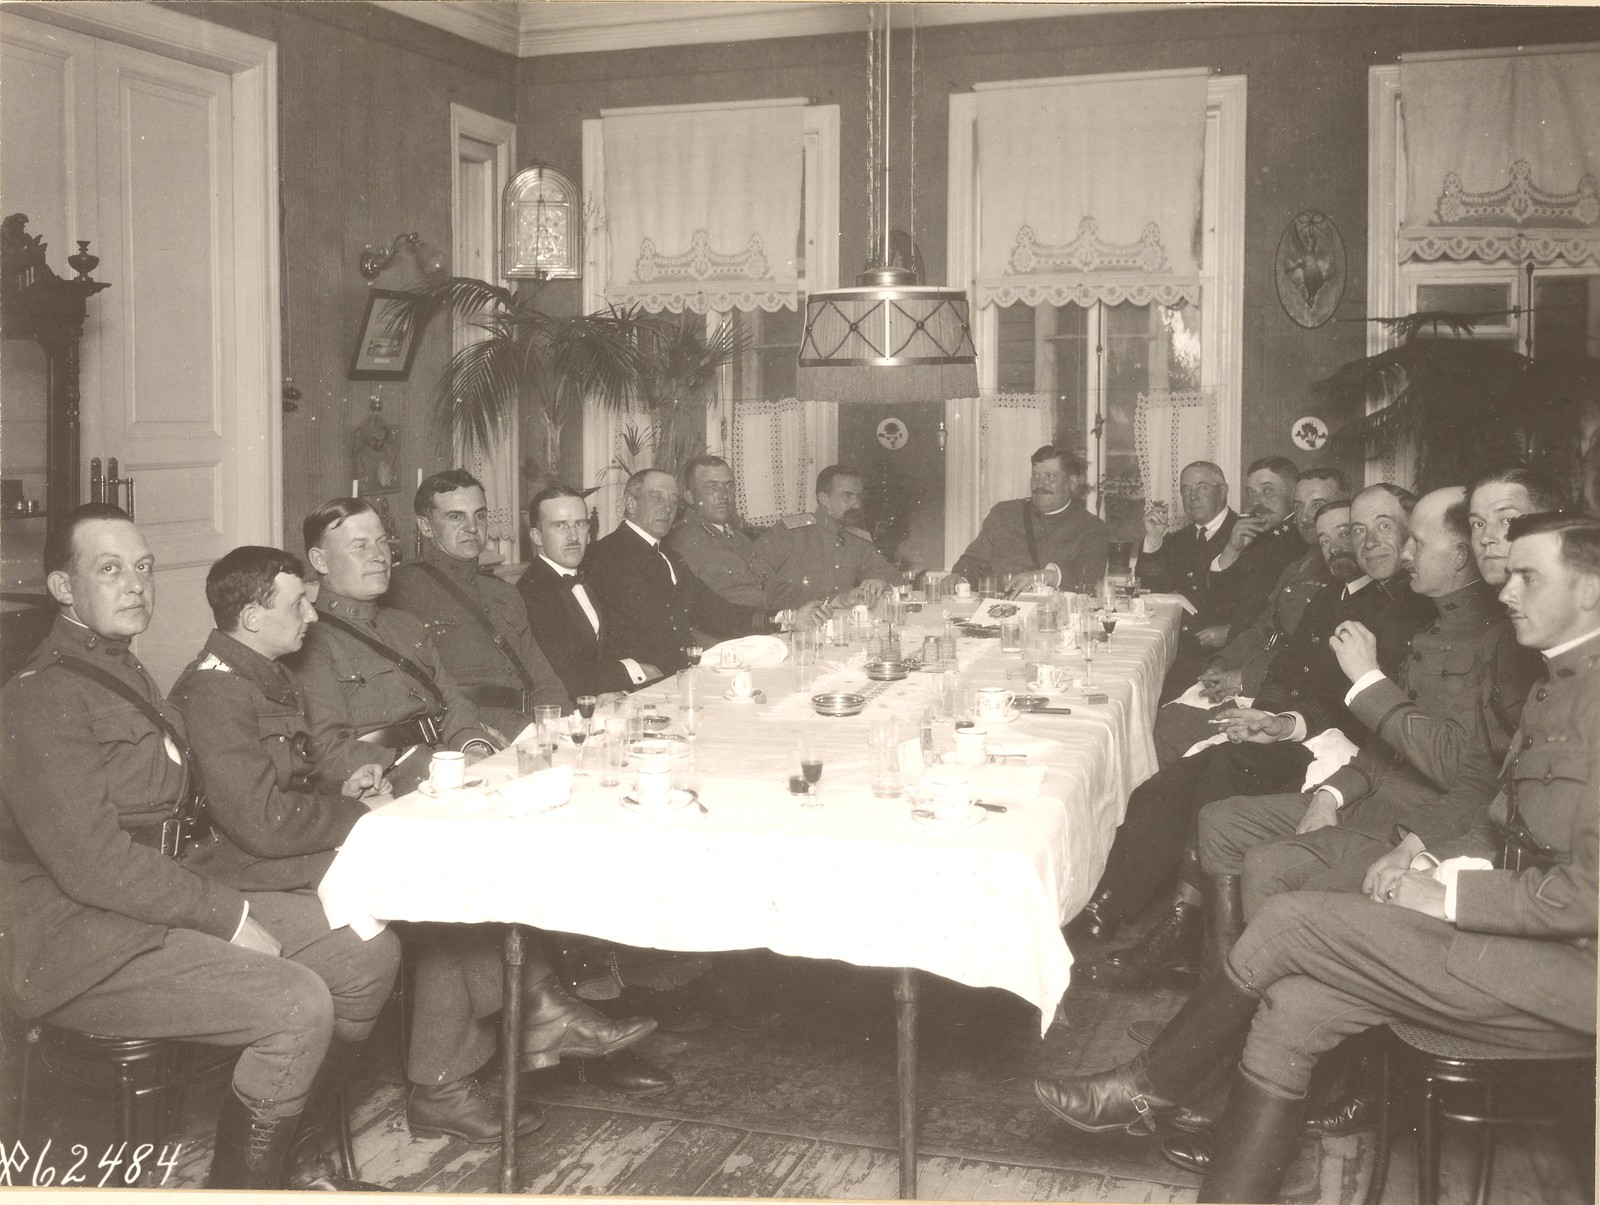
\includegraphics[width=.95\columnwidth]{images/Banquet.png} 
  \end{center}

  \answer{\begin{itemize} \item In reality, “Wilson did want to avoid making the anti-Bolshevik thrust of the military expedition obvious and explicit, but it was implicit from the beginning.” \vspace{-5pt} \item On September 4, 1918, American troops landed in Arkhangelsk, as promised \vspace{-5pt} \item Murmansk and Arkhangelsk became “an indispensable corollary of Allied intervention in Siberia.” \vspace{-5pt} \item Wilson supported efforts, as long as there was “sympathy of the Russian people” \vspace{-5pt} \item American Ambassador David Francis, a staunch anti-Bolshevik, made clear (and supported) that American troops were not just sitting in Arkhangelsk  \end{itemize}}

\end{multicols}

\begin{multicols}{2}

  \answer{\begin{itemize} \item French and British overly-aggressive towards Bolsheviks, more than the U.S.\ was willing to promote \vspace{-5pt} \item The fact that Allied troops stayed for nearly a year past the end of first World War demonstrates that combating Germans was never the prime goal  \end{itemize}}

  \begin{center}
    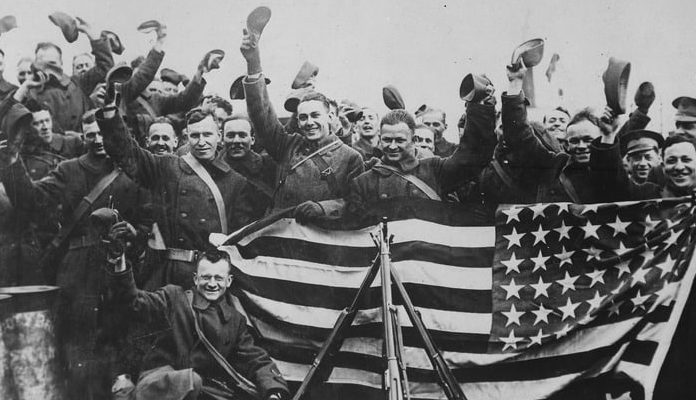
\includegraphics[width=.95\columnwidth]{images/Withdrawal.png}
  \end{center}

\end{multicols}

\vspace{-47pt}

\assignmentSection{Conclusion}

\vspace{-20pt}

\begin{multicols}{2}

  \answer{\begin{itemize} \vspace{-3pt} \item “The Government of the United States has never recognized the Bolshevik authorities and does not consider that its efforts to safeguard supplies at Archangel or to help the Czechs in Siberia have created a state of war with the Bolsheviki.`` \vspace{-7pt} \item This most accurately portrays American attitudes towards Bolsheviks \end{itemize}}

  \answer{\begin{itemize} \item Despite its less aggressive stance, America still wanted to prevent Bolsheviks from maintaining power \vspace{-7pt} \item American troops in Southward expeditions were thanks to Francis' extreme anti-Bolshevism \vspace{-7pt} \item Although initially to combat Germans, a main goal of the intervention was clearly to combat Bolshevism  \end{itemize}}

\end{multicols}

\end{document}
